% test setup
The \gls{rs} app was built and installed on three units to test on a variation of devices.
The devices were a Sony Xperia Z2, a Samsung Galaxy S6 and a Huawei Nexus 6P, all with Android Marshmallow 6.0.1 as operating system.
The app was opened and the necessary permissions were granted, so that the app could function properly.
The app was configured with the values seen in Table \ref{tab:appconfig}.

\begin{table}[!ht]
	\centering
	\begin{tabular}{l r l}
		Variable description & Value & Unit\\
		\hline
		Fastest location update interval & 60000 & milliseconds\\
		Target location update interval & 60000 & milliseconds\\ 
		Activity confidence value & 80 & percent\\
		Activity stop threshold & 180000 & milliseconds\\
		Minimum number of route locations & 4 & locations \\
		Request activity updates & 5000 & milliseconds\\ 
	\end{tabular}
	\caption{Parameter configuration in test of the background service route tracking.}
	\label{tab:appconfig}
\end{table}

% route plan
The route driven to test the location gathering can be seen in Figure \ref{fig:testroute}.
The route was driven with the intention of gathering the whole route as a single route on each of the devices.
The drive had one stop at the point marked by a green square in Figure \ref{fig:testroute}.
The stop had a duration of two minutes, thus not passing the threshold value of three minutes.
The drive continued and ended at the start position, where the persons of the respective devices walked from the vehicle to the group room.

\begin{figure}[h]
	\begin{subfigure}[b]{0.55\textwidth}
		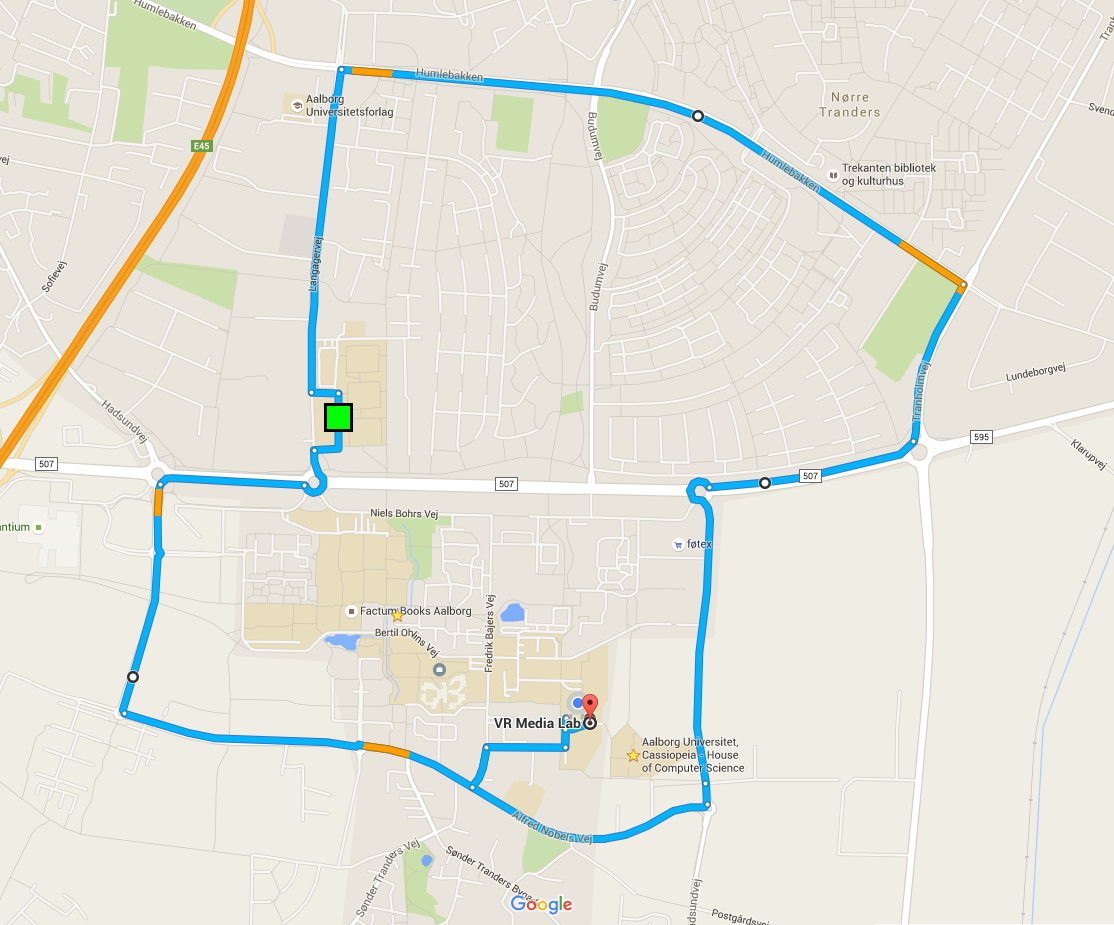
\includegraphics[width=\textwidth, trim={0 0 1cm 0},clip]{figures/testroute.png}
		\caption{Test drive route, driven clockwise from the red pin.}
		\label{fig:testroute}
	\end{subfigure}
	\begin{subfigure}[b]{0.44\textwidth}
		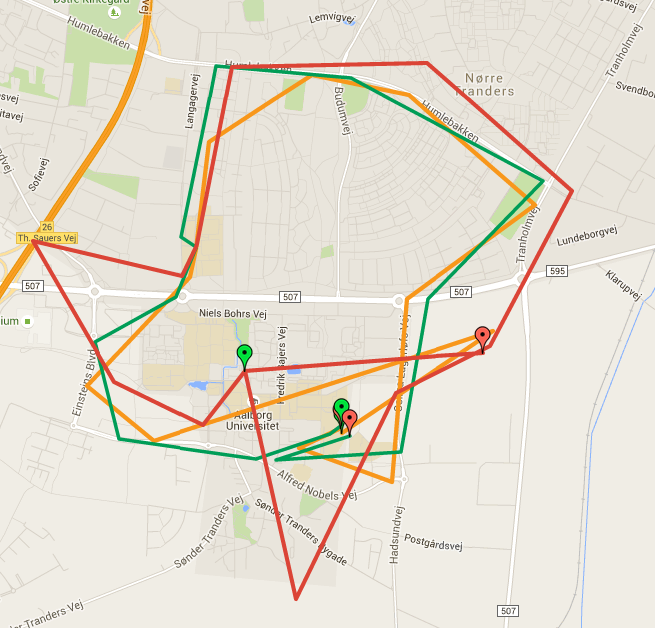
\includegraphics[width=\textwidth, trim={0 0 2cm 1.2cm},clip]{figures/testRouteRecordings.png}
		\caption{Recorded routes. Orange route is Nexus 6P, red route is Xperia Z2 and green route is Galaxy S6.}
		\label{fig:testrouterecordings}
	\end{subfigure}
	\caption{Actual route and recorded route data.}
\end{figure}

% test results
All three devices were able to gather the driven route. 
The routes were recorded with approximately the same start and end time, and the recorded routes can be seen in Figure \ref{fig:testrouterecordings}. 
As the figure shows, the gathered route data relatively accurately represent the actual route.


The Xperia device had the largest deviation from the actual route, and this could be caused by multiple factors.
Because the device was placed below the debugging laptop, interference with the GPS signals could occur.
The device could also have a poorly manufactured GPS unit.
This is not further investigated, as the two other devices gathered fairly accurate locations during the test.



% results evaluation
The test reveals that the app is able to gather locations whilst the app is not actively being utilized by a user.
The location accuracy seems to be device specific.
Location gathering as a background service is considered accomplished and the respective requirement is evaluated as fulfilled.
